\documentclass[../piano-di-progetto.tex]{subfiles}

\begin{document}

  \subsection{Consolidamento dei requisiti}

  \subsubsection{Prospetto orario}
  Nella macro-fase di Consolidamento dei requisiti, la distribuzione oraria è la seguente:
  \begin{table}[H]
    \centering
    \begin{tabular}{lccccccc}
      Nominativo                & Re         & Am         & An          & Pt         & Pr         & Ve          & Ore totali  \\
      Sofia Bononi              & 3          & -          & -           & -          & -          & 4           & 7           \\
      Enrico Buratto            & -          & -          & 3           & -          & -          & 4           & 7           \\
      Ian Nicolas Di Menna      & -          & 6          & -           & -          & -          & -           & 6           \\
      Alessandro Franchin       & -          & 3          & 4           & -          & -          & -           & 7           \\
      Enrico Galdeman           & -          & -          & 4           & -          & -          & 3           & 7           \\
      Nicholas Miazzo           & -          & -          & 4           & -          & -          & 3           & 7           \\
      Marco Nardelotto          & 3          & -          & -           & -          & -          & 4           & 7           \\
      \textbf{Ore totali ruolo} & \textbf{6} & \textbf{9} & \textbf{15} & \textbf{0} & \textbf{0} & \textbf{18} & \textbf{48}
      
    \end{tabular}
    \caption{Distribuzione oraria della macro-fase di Consolidamento dei requisiti}
  \end{table}


  Per facilitare la lettura della distribuzione oraria, i dati vengono rappresentati graficamente il seguente istogramma:
  \begin{figure}[H]
    \centering
    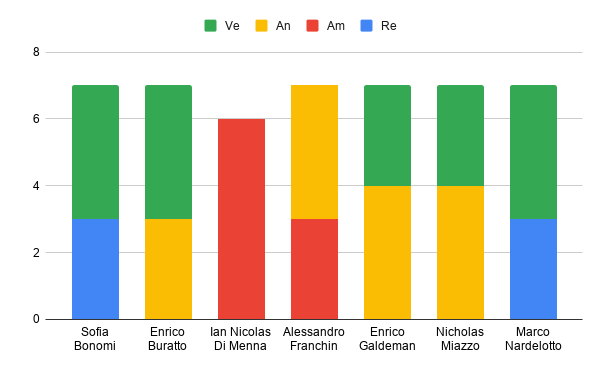
\includegraphics[width=12cm]{img/ore-consolidamento.png}
    \caption{Istogramma della distribuzione oraria della macro-fase di Consolidamento dei requisiti}
    \label{fig:ore-componente-consolidamento}
  \end{figure}

  \subsubsection{Prospetto economico}
  In questa macro-fase, la suddivisione oraria e i costi per ruolo è la seguente:

  \begin{table}[H]
    \centering
    \begin{tabular}{lcc}
      Ruolo          & Ore previste & Costo      \\
      Responsabile   & 6            & € 180,00   \\
      Amministratore & 9            & € 180,00   \\
      Analista       & 15           & € 375,00   \\
      Progettista    & -            & € 0,00     \\
      Programmatore  & -            & € 0,00     \\
      Verificatore   & 18           & € 270,00   \\
      Totale         & \textbf{48}           & \textbf{€ 1.005,00}
    \end{tabular}
    \caption{Prospetto economico della macro-fase di Consolidamento dei requisiti}
  \end{table}


  Per facilitare la lettura della suddivisione oraria per ruolo, i dati vengono rappresentati graficamente mediante il seguente areogramma:
  \begin{figure}[H]
    \centering
    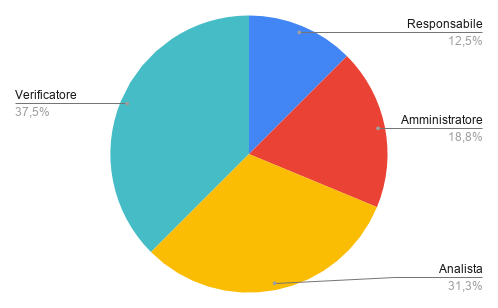
\includegraphics[width=12cm]{img/ruoli-consolidamento.png}
    \caption{Areogramma della suddivisione dei ruoli della macro-fase di Consolidamento dei requisiti}
    \label{fig:ore-ruolo-consolidamento}
  \end{figure}

\end{document}
